\clearpage


\section{Relevant text detection}
\label{cp4:corpus-relevant-text}




Next, we need text in a set of artifacts that could provide information that assists a developer solving her task.
In our corpus, this text represents \textit{golden data} that one can use to design and evaluate  
automatic tools that assist developers in the identification of  information useful to their tasks. 




To produce golden data, we follow the footsteps studies that 
ask human annotators to
mark the text that they deem useful and that provide information that could assist task completion~\cite{nadi2020, Robillard2015, marques2020}.
Overall, 
the \acs{DS-android} corpus consists of  
12,401 unique sentences
originating from artifacts associated to 50 Android development tasks and 
marked by three annotators as being relevant (or not)
to a task, as the following sections further detail. 


% \begin{itemize}
%     \item reliable golden data in a small yet diverse set of tasks and artifact types, including miscellaneous sources, which can provide new opportunities for the design of techniques that automatically detect text relevant to a task across different artifact types; and over
%     \item automatically produced golden data in a large number of
%     task and well-known artifact types where the relevant text detected by automatic approaches can serves as
%     baseline for comparison.
% \end{itemize}



\subsection{Tasks and artifacts}




We restrict the manual identification of text relevant to a task to a random subset of 
50  out of the 300 initially gathered tasks (Section~\ref{cp4:corpus-tasks}).
This decision was motivated by the fact that 
creating golden data for the entirety of our tasks 
would require asking human evaluators to inspect thousands of artifacts and more than 260,000 sentences, which would be a costly and time consuming activity. 



For each one of the tasks in this set (i.e., 25 GitHub tasks and 25 Stack Overflow tasks), we randomly selected 
one API document, a GitHub issue discussion, one Stack Overflow answer, as well as two  miscellaneous artifacts for a maximum of 5 artifacts per task for inspection.
Overall, 

comprises the inspection of 
12,401 unique sentences with an average of 63.59 sentences ($\pm 66.28$) per artifact 


\gm{There is no evaluation, so use annotators not
evaluators}
\art{updated}

We asked human annotators to read the content of these
artifacts and 
to mark sentences that they deemed useful and that provide information that assisted task completion---instructions similar to the ones used for the creation of the 
data in the \acs{DS-synthetic} corpus~\cite{marques2020}.
Since individuals might use different criteria to
assess relevance~\cite{Barry1994, Barry1998, Freund2015},
there is a risk that
the text selected by annotators does not overlap~\cite{Freund2013, Freund2015}.
Due to this reason, golden data in \acs{DS-android-small} consists of any sentence marked by annotators. 

% Section~\ref{cp4:threats} further details threats that might arise from this decision.



% Additionally, the text selected by a single annotator may still be crucial for task completion~\cite{marques2020}.


\subsubsection{Annotators}
\textcolor{white}{force ident} % this is just for the chapter outline

--- We recruited \red{n} graduate students with professional programming experience to produce \textit{golden} data for our tasks sample. \vspace{3mm}


\subsubsection{Annotation procedures}

\gm{Is this goal consistent with what the
original techniques sought to do as well?} \art{rephrased to be consistent with the original techniques}

\gm{Doesn't each annotator get each of the 10
tasks so there is no randomly assigned task?}
\art{Sorry. I missed this paragraph}

Our intention is that golden data reflect text that instruct developers to perform important actions to accomplish their task~\cite{Robillard2015, Lotufo2012}.
To produce such data, annotators had task descriptions and links to artifacts pertinent to the respective task at their disposal. We asked annotators to write a short plan (250 words max~\cite{Rastkar2010}) with instructions that a developer could follow to successfully complete the task. 
The purpose of the plan was to ensure that annotators built enough context about the task.
While perusing artifacts, annotators also had to manually highlight sentences that they deemed useful and that provided information that assisted task completion. 


The annotation process was facilitated by an in-house tool---in the form of a Web browser plugin shown in Figure~\ref{fig:corpus-annotation-tool}. In the figure, the top-right corner panel shows the browser extension. Annotators could start an annotation session and click the highlight button.
This would instrument the HTML of a page and identify each sentence in a paragraph. The tool allowed annotators to hove over individual sentences and select them as relevant (text in orange) by clicking on the hovered text. For example, the figure depicts that an annotator selected  the sentence
``\textit{Call {\small \texttt{ActivityOptions.setLockTaskEnabled()}} ... when starting the activity}'' as relevant for the lock mode task.


\begin{figure}
    \centering
    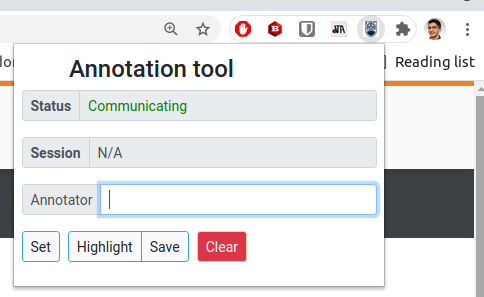
\includegraphics[width=\textwidth]{cp4/annotation-tool}
    \caption{Annotation tool and relevant sentences marked by an annotator}
    \label{fig:corpus-annotation-tool}
\end{figure}


\subsubsection{Results}

--- Provide summary of size of \acs{DS-android-small}. 

--- Descriptive statistics for marked sentences, similar to ICPC paper

--- State how the manually produced data can be used for the evaluation newly developed
techniques






\subsubsection{Metrics}

To compute an approach's accuracy, we use standard \textit{precision} and \textit{recall} metrics~\cite{Manning2009IR} and the text marked by the human annotators in \acs{DS-android-small}.
Since the text marked by them varies, we compute metrics when the manually produced golden data consists of the text marked by one, two, or the three annotators (i.e., $n=1, 2,$ or $3$).

\gm{I am not quite following ratio here...}
\art{I removed references to ratio and started using accuracy}



To ease interpreting precision and recall, Table~\ref{tbl:type-I-II-errors} show all possible evaluation outcomes. The \textit{relevant} and \textit{not-relevant} columns represent the text 
marked (or not) by the annotators. Rows represent the text automatically identified by an automatic approach.


\begin{table}[H]
\centering    
\begin{scriptsize}
\begin{threeparttable}
\begin{tabular}{l|l|l}

\hline

\textbf{}
& \textbf{Relevant}    
& \textbf{Not-relevant} \\

\hline
\hline

\textbf{Identified as relevant} & true positive ($TP$) & false positive ($FP$) \\
\hline
\textbf{Identified as Not-relevant} & false negative ($FN$) & true negative ($TN$) \\
\hline

\end{tabular}
\end{threeparttable}
\end{scriptsize}
\caption{Result outcomes}
\label{tbl:type-I-II-errors}
\end{table}

    



For a given task $t$ and artifact $a$, $precision_n$ is the fraction of the sentences identified that are marked as relevant by $n$ annotators over the total number of sentences identified, as shown in Equation~\ref{eq:cp4:precision}. For example, \textit{precision(t, API documentation)\textsubscript{2}} computes the number of sentences identified by \acs{Krec} for the task $t$ when 
golden data consist of sentences marked by two or more annotators.


\begin{equation}
\label{eq:cp4:precision}    
    Precision(t, a)_n = \frac{TP}{TP + FP}
\end{equation}


Recall ($recall_n$) represents how many of all sentences marked by at least $n$ annotators are identified by a technique (Equation~\ref{eq:cp4:recall}).


\begin{equation}
\label{eq:cp4:recall}        
    Recall(t, a)_n = \frac{TP}{TP + FN}
\end{equation}

% \vspace{3mm}




% \subsection{Results}
% \textcolor{white}{force ident} % this is just for the chapter outline


% --- Discuss results.\footnote{\red{think which summary tables should I have in the thesis body and which I can move to Appendices}} \vspace{3mm}



% --- Precision~\ref{tbl:ds-small-results-precision}  \vspace{3mm}


% --- Recall~\ref{tbl:ds-small-results-recall} \vspace{3mm}

% --- Likely explanation for the results obtained.

% % When interpreting results, we favor precision instead of recall.
% % A false positives may contribute to a developer abandoning reading of an artifact that would otherwise provide crucial information for her task~\cite{Rastkar2010}.




% \begin{table}[H]
\centering    
\begin{scriptsize}
\begin{threeparttable}
\begin{tabular}{lcccccc}

\hline


\multirow{2.5}{*}{Technique}
& \multicolumn{2}{c}{\textit{$Precision_{n=3}$}}
& \multicolumn{2}{c}{\textit{$Precision_{n=2}$}}
& \multicolumn{2}{c}{\textit{$Precision_{n=1}$}}
\\ \cmidrule(l){2-3} \cmidrule(l){4-5} \cmidrule(l){6-7} 


& \textit{mean}
& \textit{std}
& \textit{mean}
& \textit{std}
& \textit{mean}
& \textit{std}
\\


\hline
\hline

\acs{AnsBot} 
& 0.5 & 0.5 % = 3
& 0.5 & 0.5 % = 2
& 0.5 & 0.5 % = 1
\\

\acs{Krec} 
& 0.5 & 0.5 % = 3
& 0.5 & 0.5 % = 2
& 0.5 & 0.5 % = 1
\\

\acs{Hurried} 
& 0.5 & 0.5 % = 3
& 0.5 & 0.5 % = 2
& 0.5 & 0.5 % = 1
\\

\hline

\end{tabular}
\end{threeparttable}
\end{scriptsize}
\caption{Precision of each technique for the tasks of \acs{DS-android-small}}
\label{tbl:ds-small-results-precision}
\end{table}

    

% \begin{table}[H]
% \centering    
% \begin{scriptsize}
% \begin{threeparttable}
% \begin{tabular}{lcccccccccccc}

% \hline


% \multirow{2.5}{*}{Technique}
% & \multicolumn{10}{c}{\textit{Tasks}} 
% & \multicolumn{2}{c}{\textit{Precision}}
% \\  \cmidrule(l){2-11} \cmidrule(l){12-13} 



% &
% \textit{T1} & \textit{T2} & \textit{T3} & \textit{T4} & \textit{T5}
% & \textit{T6} & \textit{T7} & \textit{T8} & \textit{T9} & \textit{T10}
% & \textit{mean}
% & \textit{std}
% \\


% \hline
% \hline

% \acs{AnsBot} 
% & 0.5 & 0.5 & 0.5 & 0.5 & 0.5
% & 0.5 & 0.5 & 0.5 & 0.5 & 0.5
% & 0.5 % mean
% & 0.5 % std
% \\

% \acs{Krec} 
% & 0.5 & 0.5 & 0.5 & 0.5 & 0.5
% & 0.5 & 0.5 & 0.5 & 0.5 & 0.5
% & 0.5 % mean
% & 0.5 % std
% \\

% \acs{Hurried} 
% & 0.5 & 0.5 & 0.5 & 0.5 & 0.5
% & 0.5 & 0.5 & 0.5 & 0.5 & 0.5
% & 0.5 % mean
% & 0.5 % std
% \\

% \hline

% \end{tabular}
% \end{threeparttable}
% \end{scriptsize}
% \caption{Precision of each technique for the tasks of \acs{DS-android-small}}
% \label{tbl:ds-small-results-precision}
% \end{table}

    

% \begin{table}[H]
\centering    
\begin{scriptsize}
\begin{threeparttable}
\begin{tabular}{lcccccc}

\hline


\multirow{2.5}{*}{Technique}
& \multicolumn{2}{c}{\textit{$Recall_{n=3}$}}
& \multicolumn{2}{c}{\textit{$Recall_{n=2}$}}
& \multicolumn{2}{c}{\textit{$Recall_{n=1}$}}
\\ \cmidrule(l){2-3} \cmidrule(l){4-5} \cmidrule(l){6-7} 


& \textit{mean}
& \textit{std}
& \textit{mean}
& \textit{std}
& \textit{mean}
& \textit{std}
\\


\hline
\hline

\acs{AnsBot} 
& 0.5 & 0.5 % = 3
& 0.5 & 0.5 % = 2
& 0.5 & 0.5 % = 1
\\

\acs{Krec} 
& 0.5 & 0.5 % = 3
& 0.5 & 0.5 % = 2
& 0.5 & 0.5 % = 1
\\

\acs{Hurried} 
& 0.5 & 0.5 % = 3
& 0.5 & 0.5 % = 2
& 0.5 & 0.5 % = 1
\\

\hline

\end{tabular}
\end{threeparttable}
\end{scriptsize}
\caption{Recall of each technique for the tasks of \acs{DS-android-small}}
\label{tbl:ds-small-results-recall}
\end{table}

    


% \subsection{Threats}
% \label{cp4:corpus-threats}

% --- \red{Argue that this is not a replication study but rather establishing thresholds} \vspace{3mm}

% --- Discuss threats \vspace{3mm}



